% ============================================================
%  Buffer gate - physical wiring diagram.
%  Two 2N3904 packages (flat face toward you, legs DOWN, E B C),
%  wired as two NOT stages in series: Q1 collector (= A-bar) feeds
%  Q2's base through R_B2, and Q2's collector is the output.
%  Same circuit as circuit.tex, drawn the way the parts sit.
%  Compile:  pdflatex wiring.tex
% ============================================================
\documentclass[border=12pt]{standalone}
\usepackage{circuitikz}
\usepackage{tikz}
\usetikzlibrary{calc}

\def\w{0.95}
% TO-92 package: #1 = x-centre, #2 = reference name (Q1, Q2, ...)
\newcommand{\pkg}[2]{%
  \begin{scope}[shift={(#1,0)}]
    \draw[fill=black!10] (-\w,4.2) -- (-\w,5.2) arc (180:0:\w) -- (\w,4.2) -- cycle;
    \node at (0,4.6) {\small\textbf{2N3904}};
    \node[font=\footnotesize] at (0,5.55) {#2};
    \foreach \dx in {-0.6,0,0.6}{ \draw (\dx,4.2) -- (\dx,3.5); }
    \node[red,font=\bfseries\small,left=1pt]  at (-0.6,3.85) {E};
    \node[red,font=\bfseries\small,right=1pt] at ( 0.0,3.85) {B};
    \node[red,font=\bfseries\small,right=1pt] at ( 0.6,3.85) {C};
  \end{scope}}

\begin{document}
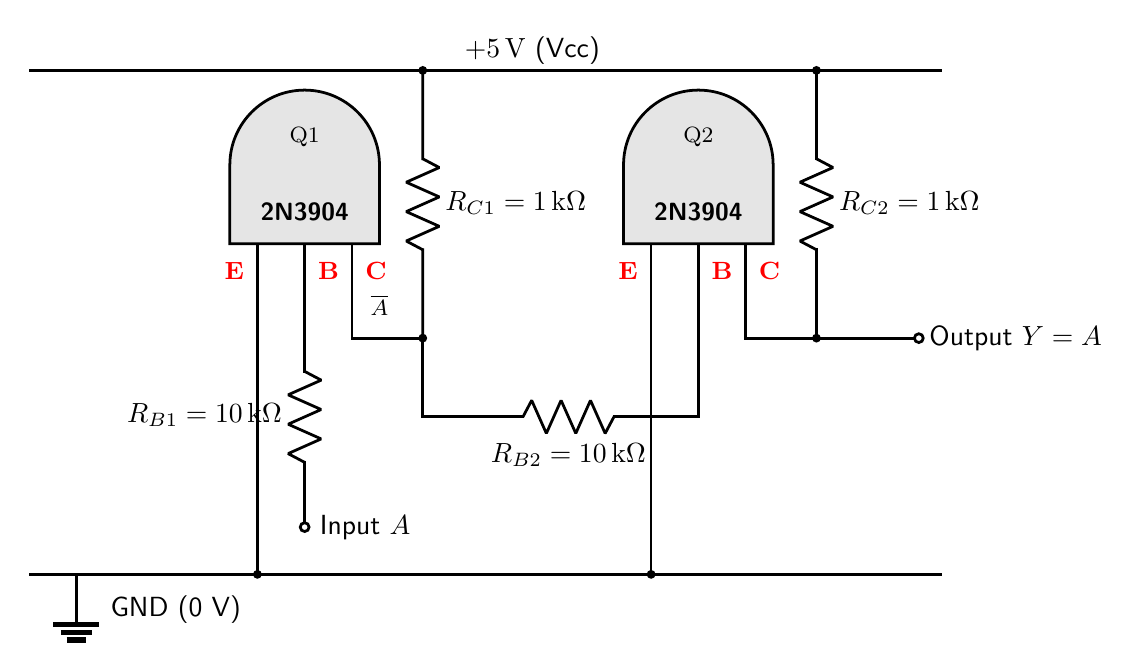
\begin{tikzpicture}[line width=1pt, font=\sffamily]
  \ctikzset{tripoles/thickness=1, bipoles/thickness=1}

  % ---------- power rails ----------
  \draw (-2,6.4) -- (9.6,6.4);
  \node[anchor=west] at (3.4,6.65) {$+5\,\mathrm{V}$ (Vcc)};
  \draw (-2,0) -- (9.6,0);
  \draw (-1.4,0) -- (-1.4,-0.05) node[ground, scale=1.4]{};
  \node[anchor=west] at (-1.1,-0.45) {GND (0 V)};

  % ---------- transistors ----------
  \pkg{1.5}{Q1}
  \pkg{6.5}{Q2}

  % ===== Q1 (NOT stage 1) =====
  % emitter -> GND rail
  \draw (0.9,3.5) -- (0.9,0);  \fill (0.9,0) circle (1.6pt);
  % base -> R_B1 -> Input A
  \draw (1.5,3.5) -- (1.5,2.9) to[R, l_={$R_{B1}=10\,\mathrm{k}\Omega$}] (1.5,1.1)
        -- (1.5,0.6) node[ocirc]{} node[right]{\,Input $A$};
  % collector -> R_C1 -> +5 V  (this node = A-bar)
  \draw (2.1,3.5) -- (2.1,3.0) -- (3.0,3.0);
  \fill (3.0,3.0) circle (1.6pt);
  \draw (3.0,3.0) to[R, l_={$R_{C1}=1\,\mathrm{k}\Omega$}] (3.0,6.4);
  \fill (3.0,6.4) circle (1.6pt);
  \node[anchor=south,font=\footnotesize] at (2.45,3.15) {$\overline{A}$};

  % ===== interstage: A-bar -> R_B2 -> Q2 base =====
  \draw (3.0,3.0) -- (3.0,2.0) -- (4.1,2.0)
        to[R, l_={$R_{B2}=10\,\mathrm{k}\Omega$}] (5.6,2.0) -- (6.5,2.0) -- (6.5,3.5);

  % ===== Q2 (NOT stage 2) =====
  % emitter -> GND rail
  \draw (5.9,3.5) -- (5.9,0);  \fill (5.9,0) circle (1.6pt);
  % collector -> R_C2 -> +5 V, and Output
  \draw (7.1,3.5) -- (7.1,3.0) -- (8.0,3.0);
  \fill (8.0,3.0) circle (1.6pt);
  \draw (8.0,3.0) to[R, l_={$R_{C2}=1\,\mathrm{k}\Omega$}] (8.0,6.4);
  \fill (8.0,6.4) circle (1.6pt);
  \draw (8.0,3.0) -- (9.3,3.0) node[ocirc]{} node[right]{Output $Y=A$};

\end{tikzpicture}
\end{document}
